\chapter{Voraussetzungen}

%	\section{Machine Learning}
	
	\section{RESTful APIs} % Raphael
	
		Representational State Transfer beschreibt ein architektonisches Modell, um Web Services zu erstellen. Sogenannte \ac{REST} Web Services bieten Interoperabilität zwischen Computersystemen im Internet -- geeignet für die Kommunikation von Maschine zu Maschine. So lässt sich REST auch als eine Abstraktion der Struktur und des Verhaltens des World Wide Webs beschreiben. 
		
		Neben REST gibt es weitere Alternativen, wie \ac{SOAP} oder \ac{RPC}; der Vorteil von REST besteht jedoch darin, dass durch das \ac{WWW} ein Großteil der Infrastruktur für die Kommunikation bereits vorhanden und implementiert ist. Während bei \\ac{RPC} in der \ac{URI} Methodeninformationen enthalten sind, gibt eine \ac{URI} in der \ac{REST} Architektur ausschließlich Ressourcen an und kodiert die Funktionalität mittels \ac{HTTP} Methoden. Dieser Ansatz entspricht dem Konzept einer \ac{URI}, da bei einer \ac{HTTP} Anfrage ebenso nur Ressourcen und keine Funktionalität gefragt ist.
		
		Eine REST API muss insgesamt sechs Eigenschaften besitzen:
		
		\begin{description}
			\item[Client-Server Architektur] 
				Bei \ac{REST} gilt im Allgemeinen, dass eine Client-Server Architektur vorliegen soll: Der Client konsumiert die vom Server bereitgestellten Dienste. 
			\item[Zustandslosigkeit] 
				Eine RESTful \ac{API} hat keine Zustände, sondern ist so konzipiert, dass benötigten Informationen in einer REST-Nachricht enthalten sind. Dies begünstigt außerdem die Skalierbarkeit eines solchen Dienstes, da es auf diese Weise einfacher ist, alle eingehenden Anfragen auf mehrere Instanzen zu verteilen.
			\item[Caching] 
				Server sowie Client können Antworten zwischenspeichern. Es muss jedoch vorher explizit definiert werden, welche Antworten zwischengespeichert und welche nicht zwischengespeichert werden, um zu verhindern, dass alte oder ungeeignete Daten versendet werden.
			\item[Einheitliche Schnittstelle]
				Die \ac{REST} \ac{API} muss eine einheitliche Schnittstelle zur Verfügung stellen, welche den von \cite{RoyThomasFielding.2000} definierten Anforderungen entsprechen muss. Dies vereinfacht die Nutzung der \ac{API}.
			\item[Mehrschichtige Systeme]
				 Die Struktur einer RESTful \ac{API} soll mehrschichtig sein, sodass es ausreicht, dem Client lediglich die oberste Schicht als Schnittstelle anzubieten. Die Architektur der API wird dadurch simplifiziert und die dahinterliegenden Schichten der Implementierung bleiben verborgen.
			\item[Code on Demand] 
				Fielding beschreibt diese Eigenschaft als optional: Der Server kann, durch das Übertragen von ausführbarem Code, die Funktionalität des Clients zeitweise erweitern oder anpassen. Vorstellbar wäre beispielsweise eine Übertragung von bereits kompilierten Komponenten oder Client-seitigen Skripten. Dies gilt es jedoch mit Vorsicht zu genießen, da diese Funktionalität auch Sicherheitslücken bergen und somit eine geeignete Angriffsmöglichkeit bieten kann. 
				
		\end{description}

	\section{Frameworks}
	
		\subsection{OpenAPI} % Raphael
		
			Der OpenAPI Standard ist Open Source und dient der Beschreibung von RESTful APIs. Bis 2016 war OpenAPI Teil des Swagger Frameworks, wurde aber schließlich als separates Projekt unter Aufsicht der sog. \textit{OpenAPI Initiative}  ausgelagert. 
			
			Mit der deklarativen Ressourcenspezifikation von OpenAPI können Clients Dienste verstehen und konsumieren, ohne über Kenntnisse der eigentlichen Server-Implementierung bzw. Zugriff auf den Servercode zu verfügen. Dies erleichtert die Entwicklung Client-seitiger Applikationen, die RESTful APIs verwenden. Die OpenAPI-Spezifikation ist zudem sprachunabhängig und lässt sich in jeder Beschreibungssprache (\ac{YAML}, \ac{XML} etc.) definieren. 
	
		\subsection{Swagger} % Raphael
		
			Swagger ist ein Framework, das sich des OpenAPI Standards bedient. Swagger bietet ein Tooling an, mit dessen Hilfe APIs spezifiziert und beschrieben werden können. Neben einem entsprechenden Editor, bietet Swagger die Möglichkeit, aus der OpenAPI Spezifikation Code zu generieren und zwar unter Verwendung unterschiedlicher Frameworks -- z.B. eine vollständige Spring Applikation -- wobei nur noch die eigentliche Implementierung der Businesslogik erforderlich ist.
			
			Des Weiteren stellt Swagger eine Web-basierte Benutzeroberfläche zur Verfügung, welche nicht nur die direkte Anbindung von Live APIs ermöglicht, sondern auch eine visuelle Dokumentation der \ac{API} darstellt. \cite{SmartBear.2020}
	
		\subsection{Spring} % Raphael
		
			Spring ist ein Open Source Framework, welches in Java geschrieben wurde. Es gilt als de facto Standard bei der Entwicklung von RESTful API, da es in der Open Source Welt viel Zuspruch und Verwendung gefunden hat. Zudem integriert Spring mit fast allen Java Umgebungen und ist somit nicht nur für Anwendungen im kleinen Maßstab, sondern eben so für Anwendungen in großen Unternehmen geeignet. \cite{Walls.20162017} 
			
			Bei der Entwicklung dieses Frameworks wurden die unter anderem in \cite{Johnson.2003} beschriebenen Design Prinzipien mithilfe der folgenden Module und deren entsprechender Funktionalität umgesetzt:
			
			\subsubsection{Dependency Injection} % Raphael
			
				Der von Martin Fowler 2004 definierte Begriff der \textit{Dependency Injection} in \cite{MartinFowler.23.01.2020} ist eine Präzisierung oder Spezialisierung des Begriffs \textit{Inversion of Control}. \ac{IoC} bezeichnet ein Paradigma, welches den Kontrollfluss einer Applikation nicht mehr der Anwendung, sondern dem Framework -- in diesem Fall Spring -- überlässt. Ein Beispiel für \ac{IoC} sind Listener (Beobachter Muster). \\
				Dependency Injection beschreibt ein Entwurfsmuster, bei welchem festgelegte Abhängigkeiten nicht zur Kompilierzeit, sondern zur Laufzeit bereitgestellt werden. Dies lässt sich einem Beispiel erläutern: Besteht bei der Initialisierung eines Objektes eine Abhängigkeit zu einem anderen Objekt, so wird diese Abhängigkeit an einem zentralen Ort hinterlegt. Wenn nun die Initialisierung dieses Objektes erfolgt, beauftragt es den sog. Injector (dt. Injezierer), die Abhängigkeit aufzulösen. \cite{MartinFowler.23.01.2020}
				
				In Spring bietet der \ac{IoC} Container mittels Reflexion ein konsistentes Werkzeug zur Konfiguration sowie Verwaltung von Java Objekten. Diese durch den Container erstellten Objekten heißen \textit{Beans}. Die Konfiguration des Containers erfolgt entweder über eine \ac{XML} Datei oder über Java Annotationen. \cite{Walls.20162017} 
				
			\subsubsection{Aspektorientierte Programmierung}
			
				\ac{AOP} beschreibt ein Paradigma und ermöglicht die klassenübergreifende Verwendung generischer Funktionalität. Dies führt zu einer starken Modularisierung und sorgt für eine klare Trennung zwischen der Anwendungslogik und der Businesslogik (Cross-cutting Concern). \cite{Wunderlich.2005} \\
				Das Schreiben von Logs stellt ein Beispiel für ein Cross-cutting Concern dar, da eine Logging-Strategie alle protokollierten Klassen und Methoden erfasst und somit durchaus mit der Anwendungs- sowie der Businesslogik in Berührung kommt. 
			
			\subsubsection{Transaktionsmanagement} % Raphael
			\label{frameworks.spring.transaktionsmanagement}
			
				Ein weiteres Beispiel für \ac{AOP} ist sog. Transaktionsmanagement. Eine Transaktion bezeichnet in der Informatik eine logische Einheit, mit dessen Hilfe Aktionen auf einer Persistenz ausgeführt werden können. Dabei ist sichergestellt, dass sobald die Transaktion fehlerfrei und vollständig abgeschlossen ist, der Datenbestand weiterhin konsistent ist. Im Umkehrschluss bedeutet das, dass eine Transaktion entweder vollständig oder gar nicht ausgeführt wird. \cite{Ozsu.2011}
			
				Das von Spring bereitgestellte Transaktionsmanagement stellt eine Abstraktion der Java Plattform dar und ist in der Lage mit globalen und verschachtelten Transaktionen sowie sog. Savepoints -- ein Punkt innerhalb einer Transaktion, zu welchem im Fehlerfall zurück gesprungen werden kann -- zu arbeiten. Außerdem lasst sich diese Abstraktion in fast allen Java Umgebungen einsetzen. Die von Java bereitgestellte Java Transaction API (\ac{JTA}) hingegen unterstützt nur globale und verschachtelte Transaktionen und erfordert zudem immer einen Applikationsserver. 
			
			\subsubsection{Model View Controller} % Raphael
			
				Das \ac{MVC} (Model View Controller) Pattern ist ein weit verbreiteter Mechanismus zur Entwicklung von Benutzeroberflächen. \ac{MVC} stellt ein Design Pattern dar, dass Kapselung sowie eine Struktur für eine Architektur von Benutzeroberflächen bietet und bei welcher jeder Bereich eine definierte Aufgabe hat. Eine Verletzung der Zuständigkeitsbereiche ist zu vermeiden. \cite{Gamma.1995}
			
				Das Pattern besagt, dass die Architektur von Benutzerschnittstellen in folgende Bereiche aufgeteilt ist: Das \textit{Model} ist für den Zugriff auf die Datenbank und die Beschaffung von Daten zuständig. Häufig ist das Model auch für die Aufbereitung der Daten zuständig. Somit liegt die meist aufwändige Logik nicht beim Client, sondern bei den Servern, welche zumeist auch mit besserer Hardware ausgestattet sind. \\
				Ein \textit{Controller} definiert die Art und Weise, wie die Benutzerschnittstelle auf die Eingaben des Benutzer reagiert. Des Weiteren ist ein Controller für das Aktualisieren der Daten im Datenmodell, aber auch auf dem View zuständig. \\
				Der \textit{View} bestimmt ausschließlich, wie die Benutzeroberfläche aussehen soll. Er enthält -- in den meisten Implementierungen -- keine Logik, sondern ist lediglich eine Definition und Anordnung der Benutzeroberflächenelemente.
				
				Spring definiert für alle Verantwortlichkeiten eigene Strategie-Interfaces, wie beispielsweise das Controller Interface, welches alle eingehenden \ac{HTTP} Requests definiert und darüber hinaus auch behandelt. 

		
		\subsection{Hibernate} % Raphael
		
			Hibernate ist ein Persistenz- und Object-relational Mapping (\ac{ORM}) Framework, das ebenfalls unter einer Open Source Lizenz veröffentlicht und in Java geschrieben ist. Hibernate bietet eine Abstraktionsstufe gegenüber relationalen Datenbankimplementationen. Mithilfe der Sprache \textit{Hibernate Query Language} und dem entsprechend konfigurierten Dialekt (z.B. MySQL Dialekt, MariaDB Dialekt etc.) werden die entsprechenden Statements erzeugt und schließlich ausgeführt. Dies ermöglicht den einfach und schnellen Umstieg von einer Datenbankimplementation auf die andere, ohne Anpassung der sich im Code befindlichen Queries. 
			
			\subsubsection{Object-relational Mapping} % Raphael
		
				Eine häufig eingesetzt Technik der Persistierung sind relationale und meist auch \ac{SQL} basierte Datenbanken wie beispielsweise MySQL oder MariaDB. Wenn jedoch die Anwendung, welche die Businesslogik enthält, der Objektorientierung folgt, kommt es zu einem Widerspruch -- dem sog. \textit{Object-relational impedance mismatch} --, welcher in den unterschiedlichen Paradigmen begründet liegt. So beschreibt die Objektrelationale Abbildung eine Technik, bei welcher sich Objekte einer objektorientierten Sprache in einer relationalen Datenbank persistieren lassen. \cite{Ireland.2009}
					
				Java bietet mit der sog. Java Persistence API (\ac{JPA}) eine Abstraktion genau zu diesem Zweck, dessen sich Hibernate auch bedient. Mittels Annotationen lassen sich Objekte mit Attributen und Methoden -- zumeist Plain Old Java Objects (\ac{POJO}s) -- auf Entitäten abbilden. Diese Annotation definieren, welche Tabelle auf welches Objekt und welche Spalte auf welches Attribute abgebildet wird. Es lassen sich außerdem die Relationen der Entitäten auf die Assoziationen der Objekte abbilden. Hibernate bzw.\ac{JPA} unterstützt 1:1, 1:N sowie N:N Relationen. Somit wird ein vollständiges Abbild der Persistenz in der Anwendung geschaffen.
				
				Die einzige Vorgabe bei der Definition der Objekte ist, dass ein parameterloser Konstruktor existieren muss. Hibernate greift auf die Attribute der Klasse mittels Reflexion zu. 
				
			\subsubsection{Transaktionsmanagement} % Raphael
			
				In Hibernate erfolgt der Zugriff auf die Persistenz über sogenannte \textit{Sessions}. Eine Session repräsentiert eine physische Verbindung zwischen der Persistenz und der Anwendung und bietet Methoden für alle Datenbestandsoperationen. Der Lebenszyklus einer \textit{Session} ist durch den Beginn und das Ende einer logischen Transaktion begrenzt. Es ist konfigurierbar, ob Hibernate das Sessionmanagement übernimmt, oder die Anwendung selbst die \textit{Sessions} öffnet und wieder schließt. So werden auch parallele Datenbankverbindung und damit auch eine Performance Verbesserung ermöglicht.
				
				Um eine Session mittels des Sessionmanagements zu erstellt, wird sich der \textit{SessionFactory} bedient, von welcher meist nur eine Instanz in der Applikation existiert. Diese beinhaltet die Konfiguration, die den Verbindungsaufbau und die Verbindung selbst definiert.
				
				Eine Session ermöglicht es eine \textit{Transaction} -- Abstraktion der Implementation von \ac{JTA} -- zu starten und zu beenden. Wie bereits in \autoref{frameworks.spring.transaktionsmanagement} beschrieben, lässt sich hierbei das Transaktionsmanagement sehr gut integrieren, sodass Spring das Starten und Beenden von Transaktionen handhabt. Dies führt zu einer Simplifizierung des Codes, der zum einen lesbarer und zum anderen einfacher wird. 
				
		\subsection{Docker} % Raphael
			
			Docker ist eine Open Source Virtualisierungssoftware, die der Isolierung von Anwendungen dient und von Docker Inc. bereitgestellt wird. Die Motivation hinter der Verwendung von Docker liegt im Deployment Prozess begründet: 
			
			Der noch vor einigen Jahren vorherrschende Auslieferungsprozess war zumeist eine Installationsanleitung, welche die einzelnen Anweisungsschritte beinhaltete, die es auszuführen galt, um die Applikation zu starten. Da dies jedoch auf Dauer zu komplex wurde, wurden Anwendungen mittels virtueller Maschinen ausgeliefert. Hierbei bestand der Vorteil darin, dass keine Abhängigkeiten o.Ä. installiert, sondern lediglich die virtuelle Maschine mit dem ausgelieferten Image gestartet werden musste. Jedoch beinhaltet ein solches Image ein vollständiges Gastbetriebssystem, dessen Größe die der Anwendung um einiges überstieg und damit nicht effizient und geeignet war. Des Weiteren stellt die Dauer des Starts einer virtuellen Maschine auch ein Problem dar. \\
			Um nun all diesen Problemen entgegenzuwirken, wurde Docker ins Leben gerufen. So werden alle Abhängigkeiten einer Anwendung in einem sog. Docker Image zusammengefasst, aus welchem wiederum Instanzen -- sog. Docker Container -- erzeugt werden. Diese leichtgewichtigen Images können nun sehr einfach ausgeliefert werden und sind darüber hinaus in der Lage, sehr schnell zu starten. \cite{ThomasClaudiusHuber.2019}
			
			Der Unterschied zwischen Docker und einer virtuellen Maschine besteht darin, dass, anstelle eines vollständigen Gastsystems, ein Docker Container sich des Betriebssystems des Hosts bedient, dem sog. Host OS. Mittels der Docker Engine wird der Zugriff auf den Kernel des Betriebssystems sichergestellt und diese bietet zudem die Möglichkeit Container zu erstellen, zu stoppen oder zu starten. \autoref{fig:dockerComparison} stellt diesen Unterschied graphisch dar. \cite{Turnbull.2014}
			
			\begin{figure}[ht!]
				\centering
				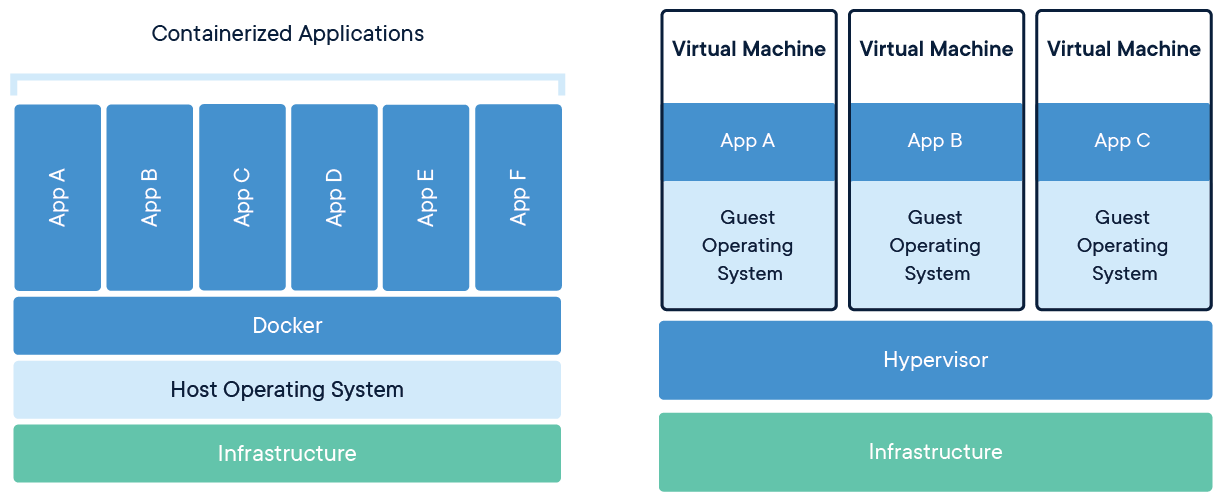
\includegraphics[width=1\textwidth]{images/docker-containerized-and-vm-transparent-bg.png}
				\caption{Docker Virtualisierung verglichen mit virtuellen Maschinen \cite{DockerInc..2020}}
				\label{fig:dockerComparison}
			\end{figure} 
			
			\subsubsection{DockerHub} % Raphael		
				
				Eine Platform, die ebenfalls von Docker Inc. bereitgestellt wird, ist der sog. DockerHub. Dieser stellt eine Registry für Docker Images und Repositories dar und bietet dem Nutzer die Möglichkeit selbst erstellte Images hochzuladen und somit anderen Nutzern zur Verfügung zu stellen. 
				
				Ferner bietet Docker eine Versionsverwaltung, welche es ermöglicht verschiedene Versionen eines Images zu erstellen. So sind die verschiedenen Versionen eines Images auf dem DockerHub einsehbar.
		
		\subsection{Android} % Raphael
	
			Google stellt für die Entwicklung von Client-Applikation auf dem Android Betriebssystem für mobile Endgeräte ein Software Development Kit \ac{SDK} zur Verfügung. Dies ermöglicht die Entwicklung von Android-Apps in den Programmiersprachen Kotlin, Java und C++. 
			
			Die Entscheidung, welche Programmiersprache zu verwenden, beschränkte sich auf Java und das auf der\ac{JVM} basierende Kotlin, da die bereits genannte Frameworks ebenfalls in Java geschrieben sind und so Einheitlichkeit herrscht. Die in \cite{AnnieDossey.2019} beschriebenen Argumente sprechen für die Verwendung von Kotlin bei der Entwicklung von Android Apps. Da Kotlin zwar ähnlich, aber nicht identisch zu Java ist, folgt aus dieser Entscheidung zudem ein Lernprozess und eine Weiterbildungsmaßnahme -- es sind keine Kenntnisse und Erfahrungen über Kotlin vorhanden --, welche im Rahmen einer wissenschaftlichen Arbeit wie dieser ausdrücklich gefordert sind.
		
			\subsubsection{Kotlin} % Raphael
			
				Kotlin ist eine plattformunabhängige und statisch typisierte Programmiersprache, die von JetBrains entwickelt wurde. Beim Kompilieren wird der Quellcode in einen Bytecode übersetzt, der unter Anderem auf der JVM laufen kann. Seit 2017 wurde Kotlin offiziell von Google für die Entwicklung von Android Apps unterstützt \cite{JetBrains.2017}. 
				
				Ein Vorteil von Kotlin gegenüber Java sing sog. Coroutines. Coroutines erleichtern die asynchrone Programmierung, indem die in Java verwendeten Callbacks -- meist durch anonyme Klassen oder seit Java 8 durch Lambdas -- ersetzt werden. Coroutines lassen sich als leichtgewichtige Threads bezeichnen und verhalten sich ähnlich wie Jobs: Auf einem Thread können mehrere Coroutines existieren und unabhängig agieren. Der Vorteil ist hierbei, dass diese deutlich performanter bzgl. Start und Erhalt sind. Zudem können Coroutines auch den aktuellen Thread zur Laufzeit mehrfach wechseln. Dies ermöglicht es, beispielsweise asynchron Daten von einer API abzurufen, und diese auf dem aktuellen UI Thread anzuzeigen und zwar innerhalb einer Coroutine, ohne den UI Thread zu blockieren. 
				
				Zu diesem Zweck hat Kotlin drei verschiedene Kontexte eingeführt unter denen eine Coroutine laufen kann:
				
				\begin{enumerate}
					\item 
						\textbf{Main:} Unter dem \textit{Main} Kontext laufen alle Operationen, die mit dem \ac{UI} interagieren. 
					\item 
						\textbf{IO}: Mithilfe des \textit{\ac{IO}} Kontextes werden Input/Output Operationen, wie beispielsweise der Zugriff auf eine Datei oder eine Web Ressource, ausgeführt.
					\item 
						\textbf{Default}: Coroutinen mit diesem Kontext stellen schwere Berechnungen an, und blockieren damit nicht den \ac{UI} Thread.
				\end{enumerate}
				
				Das Schlüsselwort \textit{suspend} in Methodenköpfen definiert, dass diese Methode in der Lage ist, asynchron zu arbeiten. Diese Methoden können entweder von weiteren \textit{suspend} Methoden aufgerufen werden, oder aber innerhalb einer Coroutine. 
		
	\section{Qualitätssichernde Maßnahmen}
	
		\subsection{Code Review}
		
		% Git, Gerrit unso dies das
	
		\subsection{Continuous Integration}
		
		\subsection{Testing Frameworks}
		                                                                                                                                                                                                                                                                                                                                         
	